\begin{frame}{}
	\maketitle
\end{frame}
\note[itemize]{
	\item
}

\begin{frame}{La torre del elefante}
	\begin{columns}
		\column[t]{0.5\textwidth}
		\begin{figure}[htb]
			\centering
			\includegraphics[width=0.4\textwidth]{img/Intro}
			\caption{Mark Schultz}
		\end{figure}
		\column[t]{0.5\textwidth}
		\begin{itemize}
			\item Una historia corta de Robert E. Howard
			\item Una de sus mejores historias
			\item Espada y hechicería (Espada y brujería) pura
		\end{itemize}
	\end{columns}
\end{frame}
\note[itemize]{
	\item
}

\begin{frame}{Publicación}
	\begin{columns}
		\column[t]{0.4\textwidth}
		\begin{figure}[htb]
			\centering
			\includegraphics[width=0.5\textwidth]{img/WeirdTales-1933-03}
			\caption{Marzo de 1933}
		\end{figure}
		\column[t]{0.6\textwidth}
		\begin{itemize}
			\item Publicada por primera vez en Weird Tales
			\item Alrededor de unas 20 páginas
			\begin{itemize}
				\item 9800 palabras en Ingles
				\item 10600 palabras en Español
				\item Lectura en 60-90 minutos
			\end{itemize}
			\item Una historia de su personaje mas famoso: Conan el bárbaro
			\item Muchas veces publicada en Español y en el idioma original
		\end{itemize}
	\end{columns}
\end{frame}
\note[itemize]{
	\item
}

\begin{frame}{La primera ilustración}
	\begin{columns}
		\column[t]{0.4\textwidth}
		\begin{figure}[htb]
			\centering
			\includegraphics[width=0.75\textwidth]{img/JayemWilcoxTowerOfTheElephant}
			\caption{Jayem Wilcox}
		\end{figure}
		\column[t]{0.6\textwidth}
		\begin{itemize}
			\item Esta ilustración acompaña a la primera edición de la historia
		\end{itemize}
	\end{columns}
\end{frame}
\note[itemize]{
	\item
}

\begin{frame}{Orden de publicación del ciclo de Conan}
	\begin{figure}[htb]
		\centering
		\includegraphics[width=0.32\textwidth]{img/OrdenPublicacion}
	\end{figure}
\end{frame}
\note[itemize]{
	\item La torre del elefante forma parte del ciclo de Conan, que consta de 18 a 25 historias de REH, dependiendo de cómo queramos contarlas.
	\item Si solo se cuentan historias publicadas en la vida de REH, son 18 (o 17 dependiendo de si se cuenta o no \say{La hija del gigante helado}).
	\item Si se añaden la historias que fueron rechazadas por los editores durante la vida de REH, y luego publicadas después de su muerte; así como fragmentos que el autor dejó inconclusos y que fueron --muchos años después-- terminados y publicados por otros autores, ahí la cuenta sube a 25.
}

\begin{frame}{Cronología ficticia del personaje}
	\begin{figure}[htb]
		\centering
		\includegraphics[width=0.85\textwidth]{img/Cronollogias}
	\end{figure}
\end{frame}
\note[itemize]{
	\item
}

\begin{frame}{Espacio en la edad Hiboria}
	\begin{figure}[htp]
		\centering
		\begin{subfigure}[b]{0.48\textwidth}
			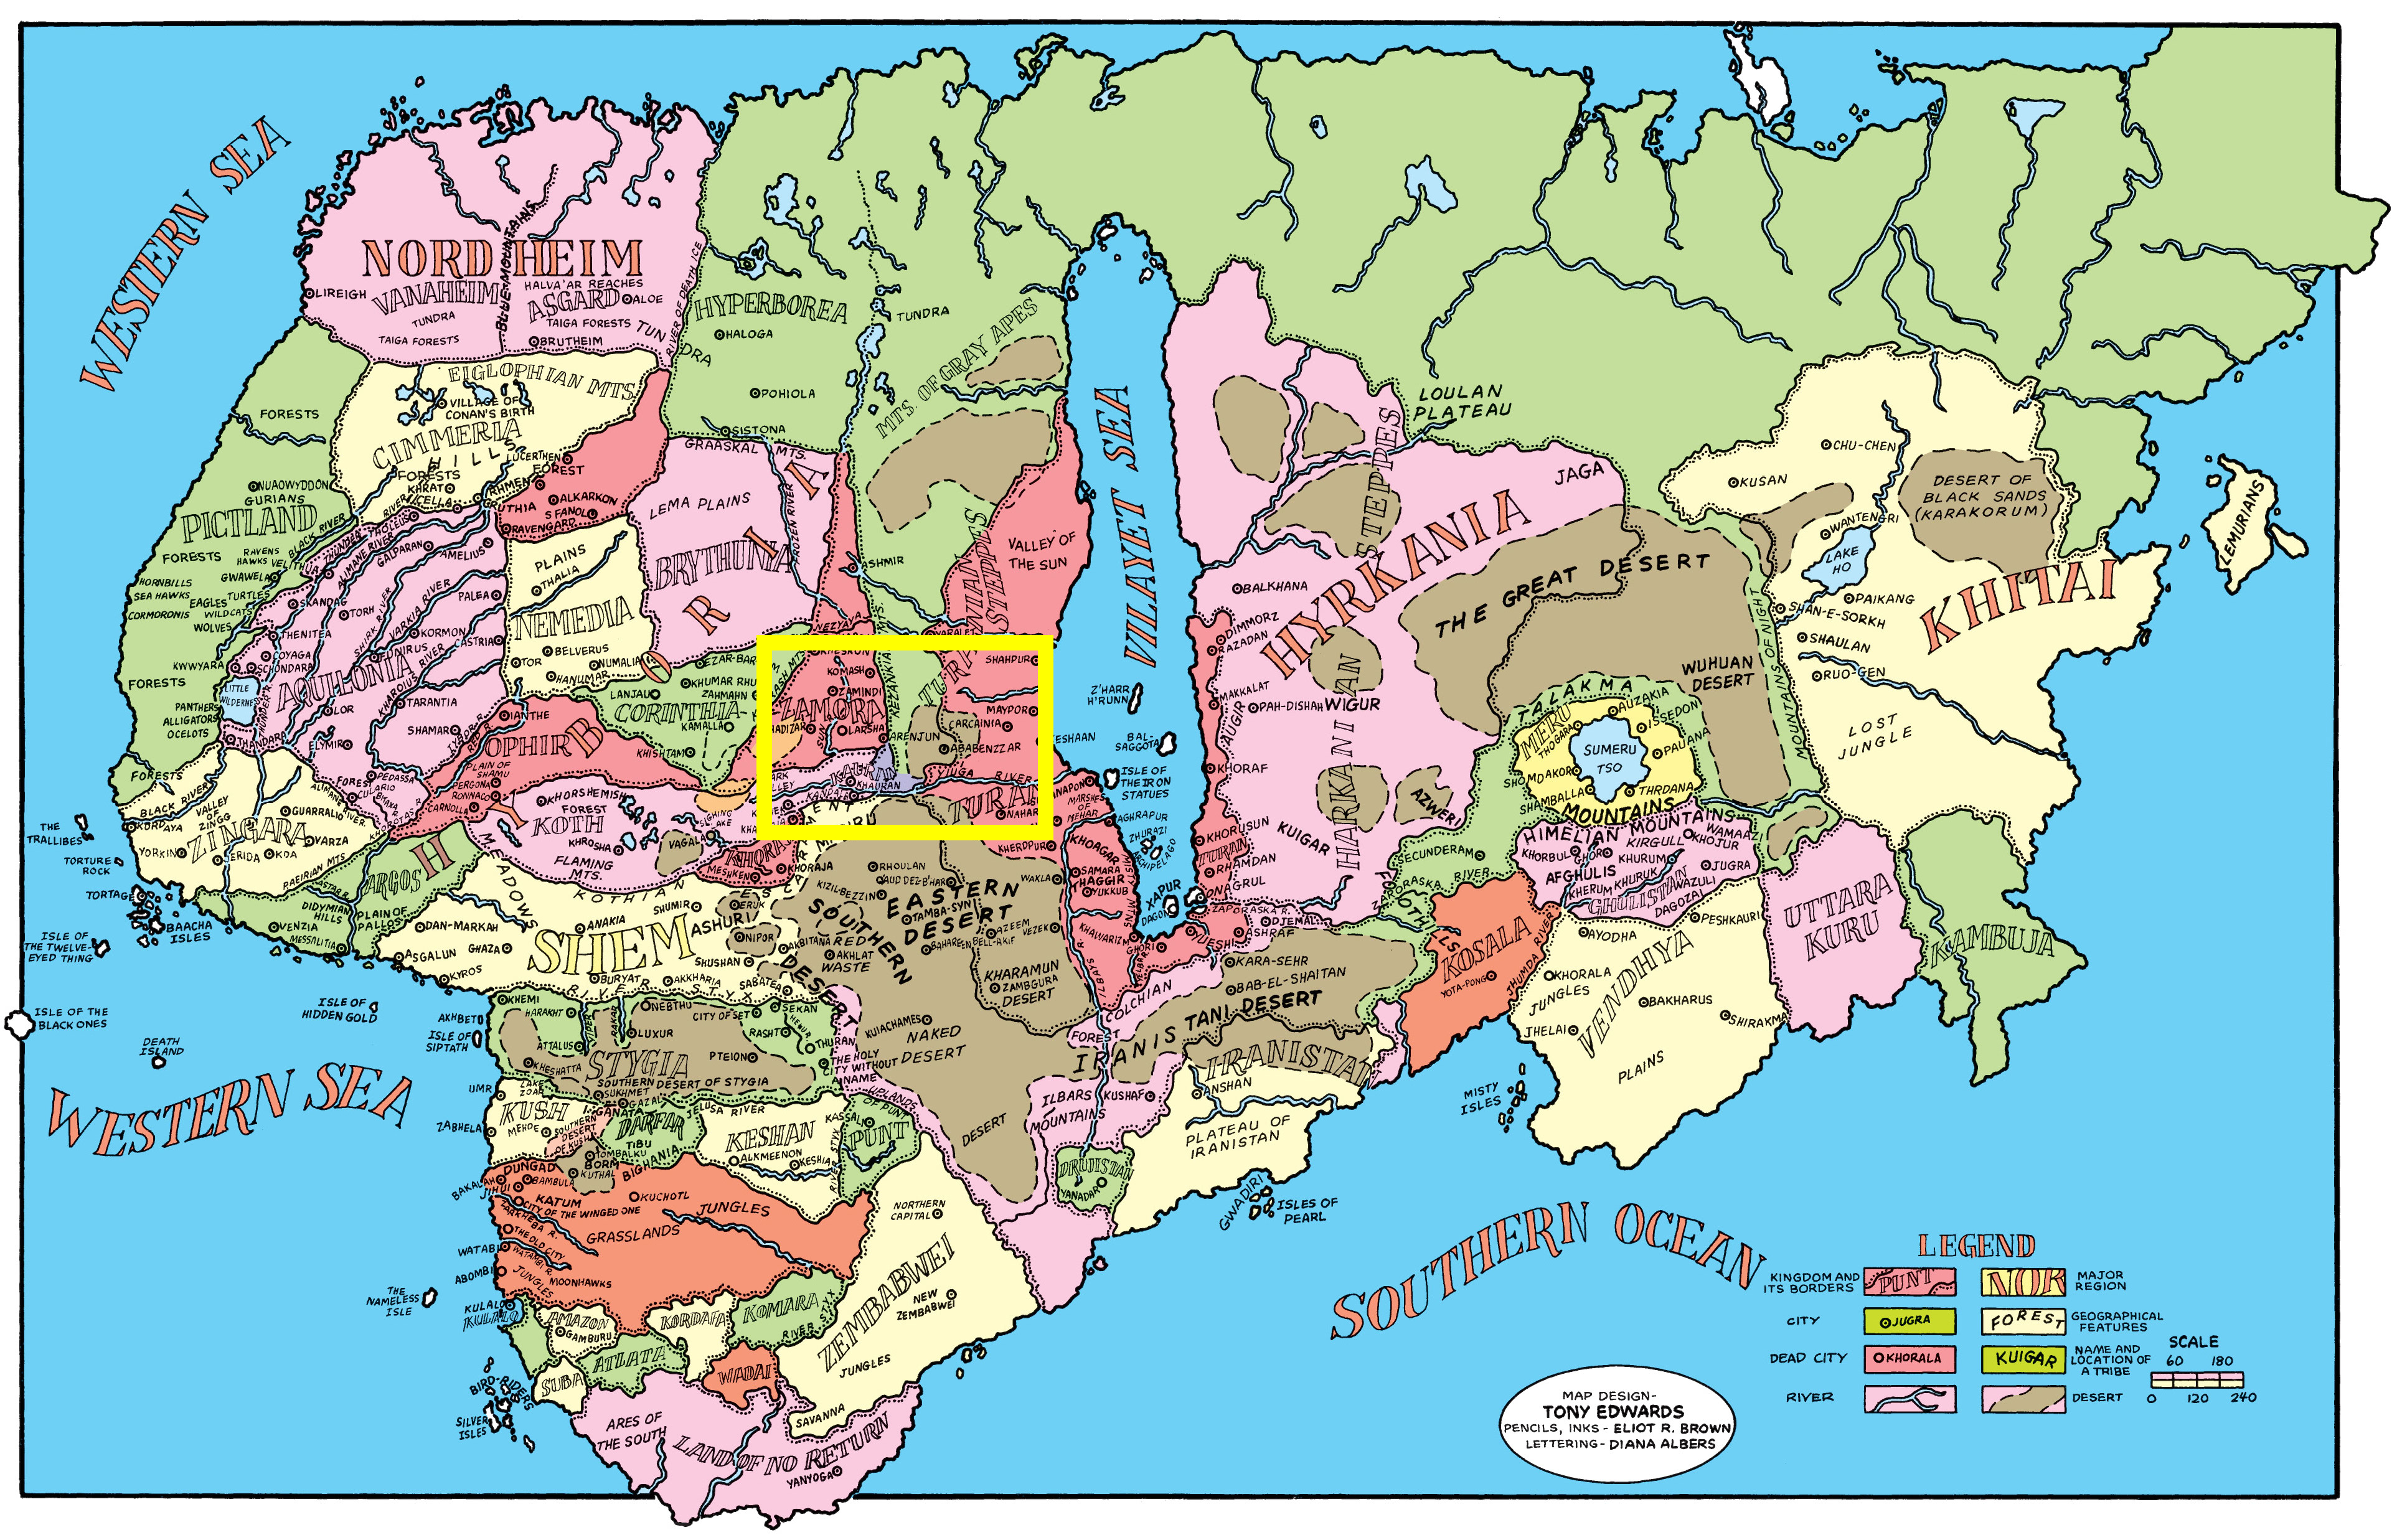
\includegraphics[width=\textwidth]{img/mapas/todo}
			%\caption{Barry Windsor Smith}
		\end{subfigure}
		~
		\begin{subfigure}[b]{0.48\textwidth}
			\includegraphics[width=\textwidth]{img/mapas/inset}
			%\caption{Silvio \say{Sal} Buscema}
		\end{subfigure}
		\caption{La ciudad de Arenjun en la provincia de Zamora. La \say{ciudad de los ladrones}}
	\end{figure}
\end{frame}
\note[itemize]{
	\item
}

\section{Adaptaciones}
\note[itemize]{
	\item
}

\begin{frame}{Conan the barbarian}
	\begin{columns}
		\column[t]{0.4\textwidth}
		\begin{figure}[htb]
			\centering
			\includegraphics[width=0.55\textwidth]{img/TheBarbarian004Portada}
			\caption{26 de Enero de 1971}
		\end{figure}
		\column[t]{0.6\textwidth}
		\begin{itemize}
			\item Número 4 en la serie
			\item 21 páginas
			\item Créditos:
			\begin{description}
				\item[Dibujante:] Barry Windsor Smith
				\item[Entintador:] Silvio \say{Sal} Buscema
				\item[Escritor:] Roy Thomas
				\item[Letrista:] Sam Rosen
				\item[Editor:] Stand Lee
			\end{description}
		\end{itemize}
	\end{columns}
\end{frame}
\note[itemize]{
	\item
}


\begin{frame}{Conan}
	\begin{columns}
		\column[t]{0.6\textwidth}
		\begin{figure}[htp]
			\centering
			\begin{subfigure}[b]{0.3\textwidth}
				\includegraphics[width=\textwidth]{img/DarkHorse20Portada}
				\caption{Septiembre}
			\end{subfigure}
			~
			\begin{subfigure}[b]{0.3\textwidth}
				\includegraphics[width=\textwidth]{img/DarkHorse21Portada}
				\caption{Octubre}
			\end{subfigure}
			~
			\begin{subfigure}[b]{0.3\textwidth}
				\includegraphics[width=\textwidth]{img/DarkHorse22Portada}
				\caption{Noviembre}
			\end{subfigure}
		\end{figure}
		\begin{center}
			2005
		\end{center}
		\column[t]{0.4\textwidth}
		\begin{itemize}
			\item \say{Conan de Dark Horse}
			\item Números 20, 21 y 22 en la serie
			\item 23, 25 y 26 pp. en cada ejemplar
			\item 20, 22 y 23 de la historia
			\item Créditos:
			\begin{description}
				\item[Artista:] Cary Nord
				\item[Artista(6pp):] Michael Kaluta
				\item[Escritor:] Kurt Busiek
				\item[Colorista:] Dave Steward
				\item[Portada:] José Ladrönn
				\item[Letrista:] Richard Starkings
			\end{description}
		\end{itemize}
	\end{columns}
\end{frame}
\note[itemize]{
	\item
}



\section{Resumen}
\note[itemize]{
	\item
}

\begin{frame}{}
	\begin{columns}
		\column[t]{0.5\textwidth}
		\begin{figure}[htb]
			\centering
			\includegraphics[width=0.9\textwidth]{img/res/01}
			\caption{El Maul}
		\end{figure}
		\column[t]{0.5\textwidth}
		\begin{figure}[htb]
			\centering
			\includegraphics[width=0.9\textwidth]{img/res/02}
			\caption{Una taberna}
		\end{figure}
	\end{columns}
\end{frame}
\note{

}


\section{Personajes}
\note[itemize]{
	\item
}

\begin{frame}{Conan}
	\begin{columns}
		\column[t]{0.4\textwidth}
		\begin{itemize}
			\item Un joven bárbaro del norte
			\item Intrépido, impulsivo y desconfiado
			\item Poco acostumbrado a la civilización
			\item Primitivo, fuerte y rebelde
		\end{itemize}
		\column[t]{0.6\textwidth}
		\begin{figure}[htp]
			\centering
			\begin{subfigure}[b]{0.3\textwidth}
				\includegraphics[width=\textwidth]{img/conan/CTB}
			\end{subfigure}
			~
			\begin{subfigure}[b]{0.27\textwidth}
				\includegraphics[width=\textwidth]{img/conan/DH}
			\end{subfigure}
			~
			\begin{subfigure}[b]{0.23\textwidth}
				\includegraphics[width=\textwidth]{img/conan/TSSC}
			\end{subfigure}
		\end{figure}
	\end{columns}
\end{frame}
\note[itemize]{
	\item
}


\section{Citas interesantes}
\note[itemize]{
	\item
}

\begin{frame}{Conan reflexiona sobre religión}
	\begin{exampleblock}{}
		He had squatted for hours in the courtyard of the philosophers, listening to the arguments of theologians and teachers, and come away in a haze of bewilderment, sure of only one thing, and that, that they were all touched in the head.
	\end{exampleblock}

	\begin{itemize}
		\item \textit{ \say{Había estado muchas horas en cuclillas en los patios de los filósofos, escuchando los razonamientos y discusiones de teólogos y maestros, y se había ido de allí confuso y perplejo y con una sola idea clara: que estaban todos locos.} }
	\end{itemize}
\end{frame}
\note[itemize]{
	\item
}


\section{Tropes literarios}
\note[itemize]{
	\item
}

\begin{frame}{Espada y hechizeria}
	\begin{columns}
		\column[t]{0.4\textwidth}
		\begin{itemize}
			\item Temporalidad: una sola noche
			\item Aventura circunstancial
			\item No genero un cambio
			\item La espada: la justicia; la hechicería: el mal
		\end{itemize}
		\column[t]{0.6\textwidth}
		\begin{figure}[htb]
			\centering
			\includegraphics[width=0.8\textwidth]{img/tributos/elephant07}
			\caption{Abe Papakhian}
		\end{figure}
	\end{columns}
\end{frame}
\note[itemize]{
	\item
}

\section{Influencias}
\note[itemize]{
	\item
}

\begin{frame}{}
	\begin{columns}
		\column[t]{0.4\textwidth}
		Hay referencias a este relato en muchos otros medios:
		\begin{itemize}
			\item El juego MMORPG: \say{wizard101 online}
			\item La serie \say{Conan the adventurer}
			\item Conan RPG de Mongoose
			\item El videojuego Conan Exiles
		\end{itemize}
		\column[t]{0.6\textwidth}
		\begin{figure}[htp]
			\centering
			\begin{subfigure}[b]{0.3\textwidth}
				\includegraphics[width=\textwidth]{img/otros/Conantheadventurerlogo}
			\end{subfigure}
			~
			\begin{subfigure}[b]{0.3\textwidth}
				\includegraphics[width=\textwidth]{img/otros/RPGgame}
			\end{subfigure}
			~
			\begin{subfigure}[b]{0.3\textwidth}
				\includegraphics[width=\textwidth]{img/otros/TowerHelephant}
			\end{subfigure}
			\\
			\begin{subfigure}[b]{0.6\textwidth}
				\includegraphics[width=\textwidth]{img/otros/trofeo}
			\end{subfigure}
		\end{figure}
	\end{columns}
\end{frame}
\note[itemize]{
	\item
}

\begin{frame}{Tributos de varios artistas}
	\begin{figure}[htp]
		\centering
		\begin{subfigure}[b]{0.22\textwidth}
			\includegraphics[width=\textwidth]{img/tributos/elephant06}
			\caption{Dai Nguyen}
		\end{subfigure}
		~
		\begin{subfigure}[b]{0.22\textwidth}
			\includegraphics[width=\textwidth]{img/tributos/elephant08}
			\caption{Spencer Sheahan}
		\end{subfigure}
		~
		\begin{subfigure}[b]{0.22\textwidth}
			\includegraphics[width=\textwidth]{img/tributos/elephant03}
			\caption{Sanjulian}
		\end{subfigure}
		~
		\begin{subfigure}[b]{0.22\textwidth}
			\includegraphics[width=\textwidth]{img/tributos/elephant04}
			\caption{Benito Gallego}
		\end{subfigure}
	\end{figure}
\end{frame}
\note[itemize]{
	\item
}

%El último slide es igual al primero: titulo y datos de contacto
\begin{frame}{}
	\maketitle
\end{frame}
